\documentclass[11pt]{article}
\usepackage[T1]{fontenc}\usepackage[utf8]{inputenc}\usepackage[brazilian]{babel}
\usepackage[a4paper,landscape,margin=1.5cm]{geometry}
\usepackage{graphicx,parskip,hyperref}
\pagestyle{plain}
\begin{document}
\section*{A — Barras: pesos e cobertura}
\begin{center}
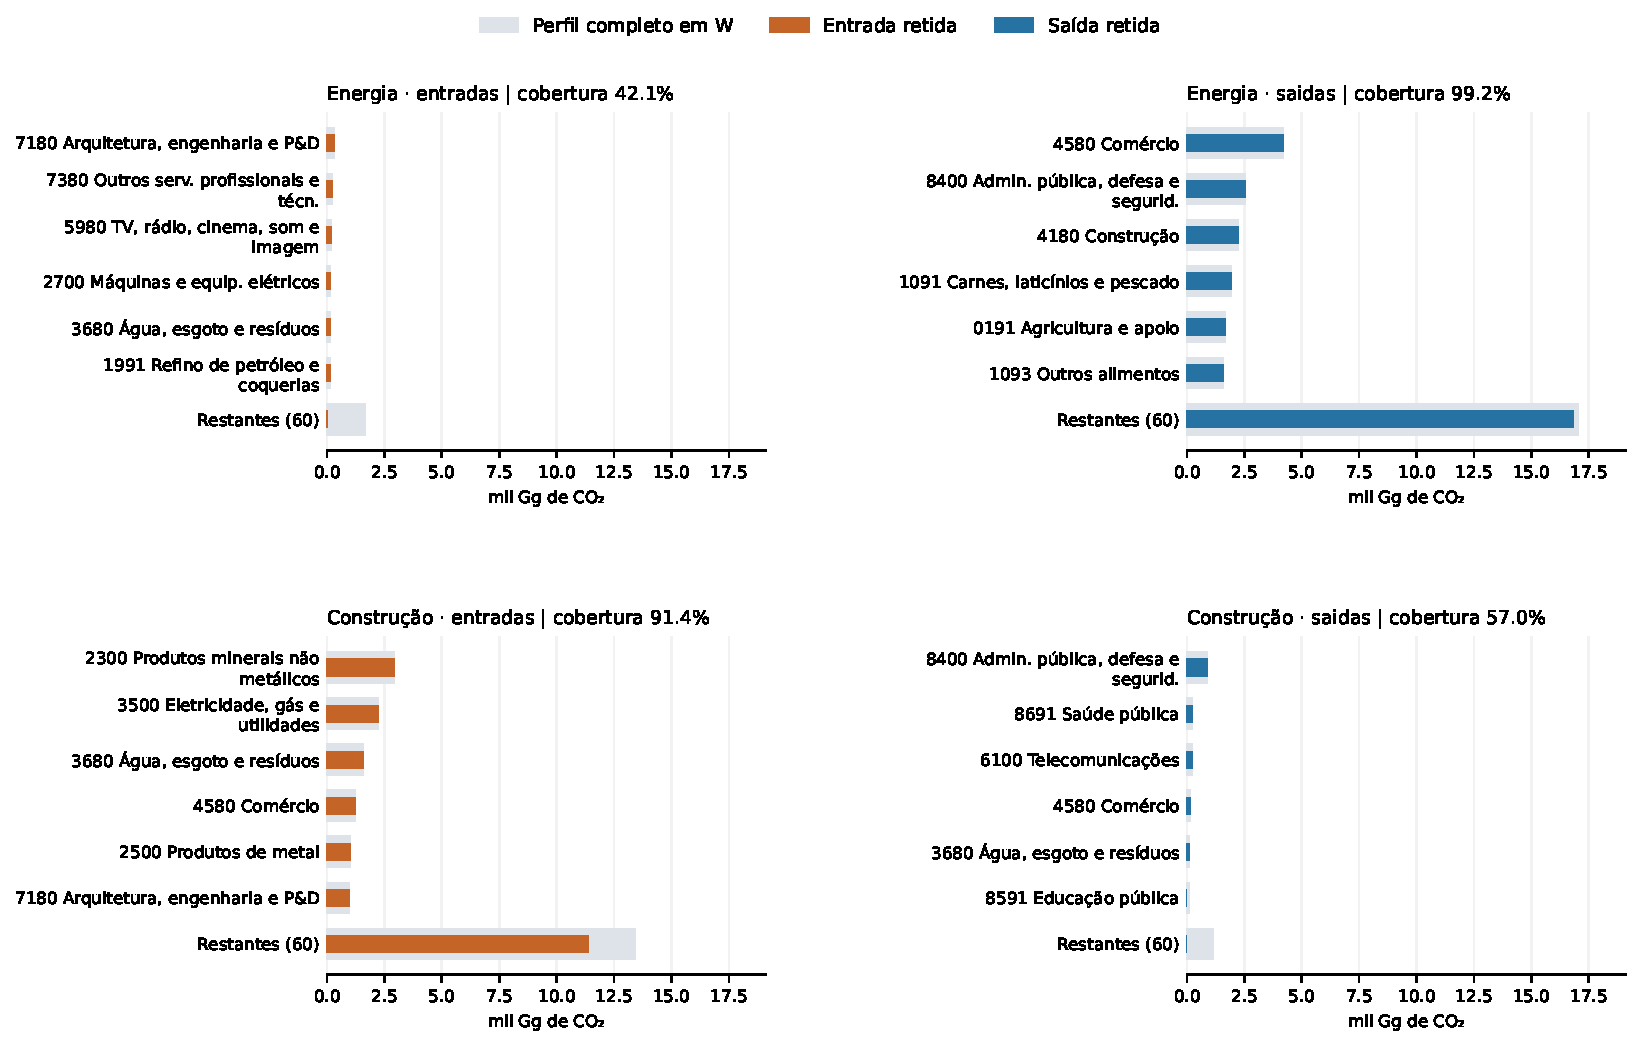
\includegraphics[width=0.96\linewidth,height=0.70\textheight,keepaspectratio]{figuras/artigo_relacoes_barras.pdf}
\end{center}
Quatro perfis. Seis maiores relações em W, mais soma das 60 restantes. Cinza: perfil completo; azul: saída retida; laranja: entrada retida. Escala comum em mil Gg de CO\textsubscript{2}. A barra restante é uma soma, não uma atividade.

Base comum: MIP brasileira de 2015, 67 atividades e intensidades aproximadas de Sanguinet e Azzoni (2024). Backbone em $\alpha=0{,}05$, pesos originais, sem diagonal. Coberturas entrada/saída: energia 42,1\%/99,2\%; construção 91,4\%/57,0\%.
\clearpage
\section*{B — Redes focais: todas as relações incidentes}
\begin{center}
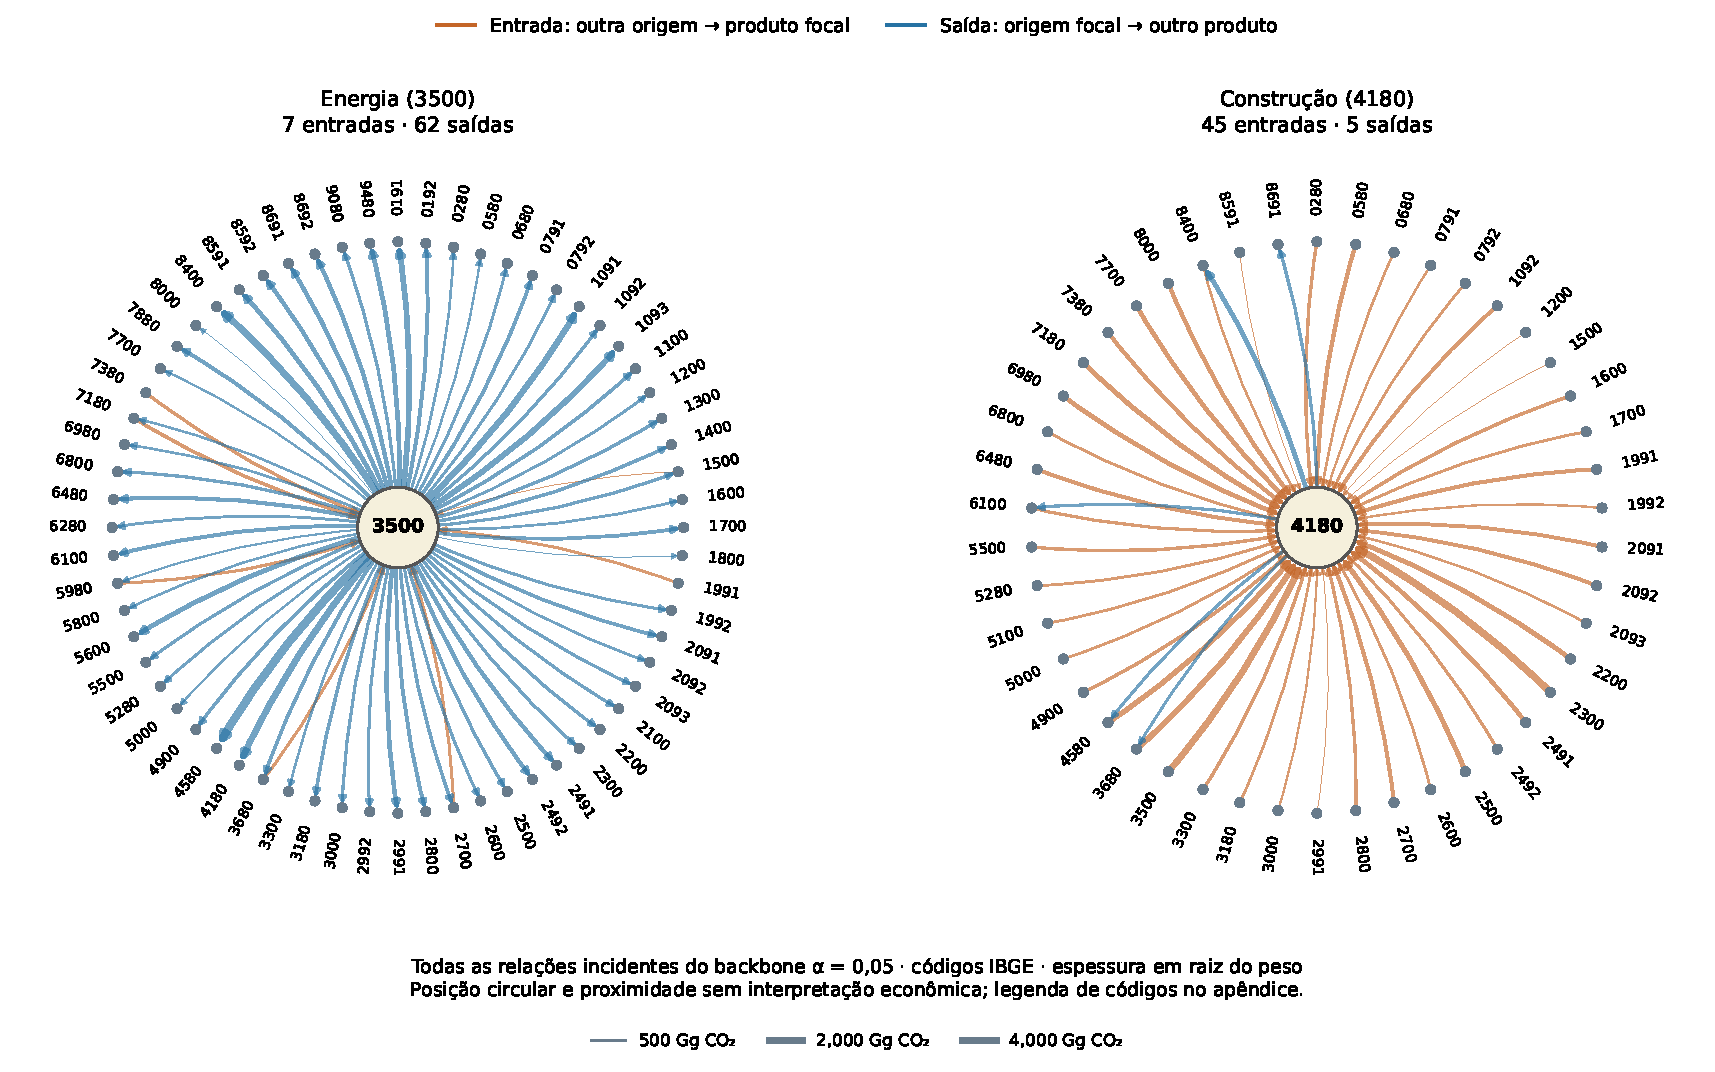
\includegraphics[width=0.96\linewidth,height=0.70\textheight,keepaspectratio]{figuras/artigo_relacoes_redes.pdf}
\end{center}
Somente relações incidentes a energia e construção no backbone; não são redes completas. Laranja: entradas; azul: saídas. Setas da origem emissora ao produto final. Mesma escala de espessura em raiz do peso; códigos IBGE conforme apêndice do artigo. Layout circular sem significado econômico.

Base comum: MIP brasileira de 2015, 67 atividades e intensidades aproximadas de Sanguinet e Azzoni (2024). Backbone em $\alpha=0{,}05$, pesos originais, sem diagonal. Coberturas entrada/saída: energia 42,1\%/99,2\%; construção 91,4\%/57,0\%.
\clearpage
\section*{C — Redes focais e barras dos sentidos predominantes}
\begin{center}
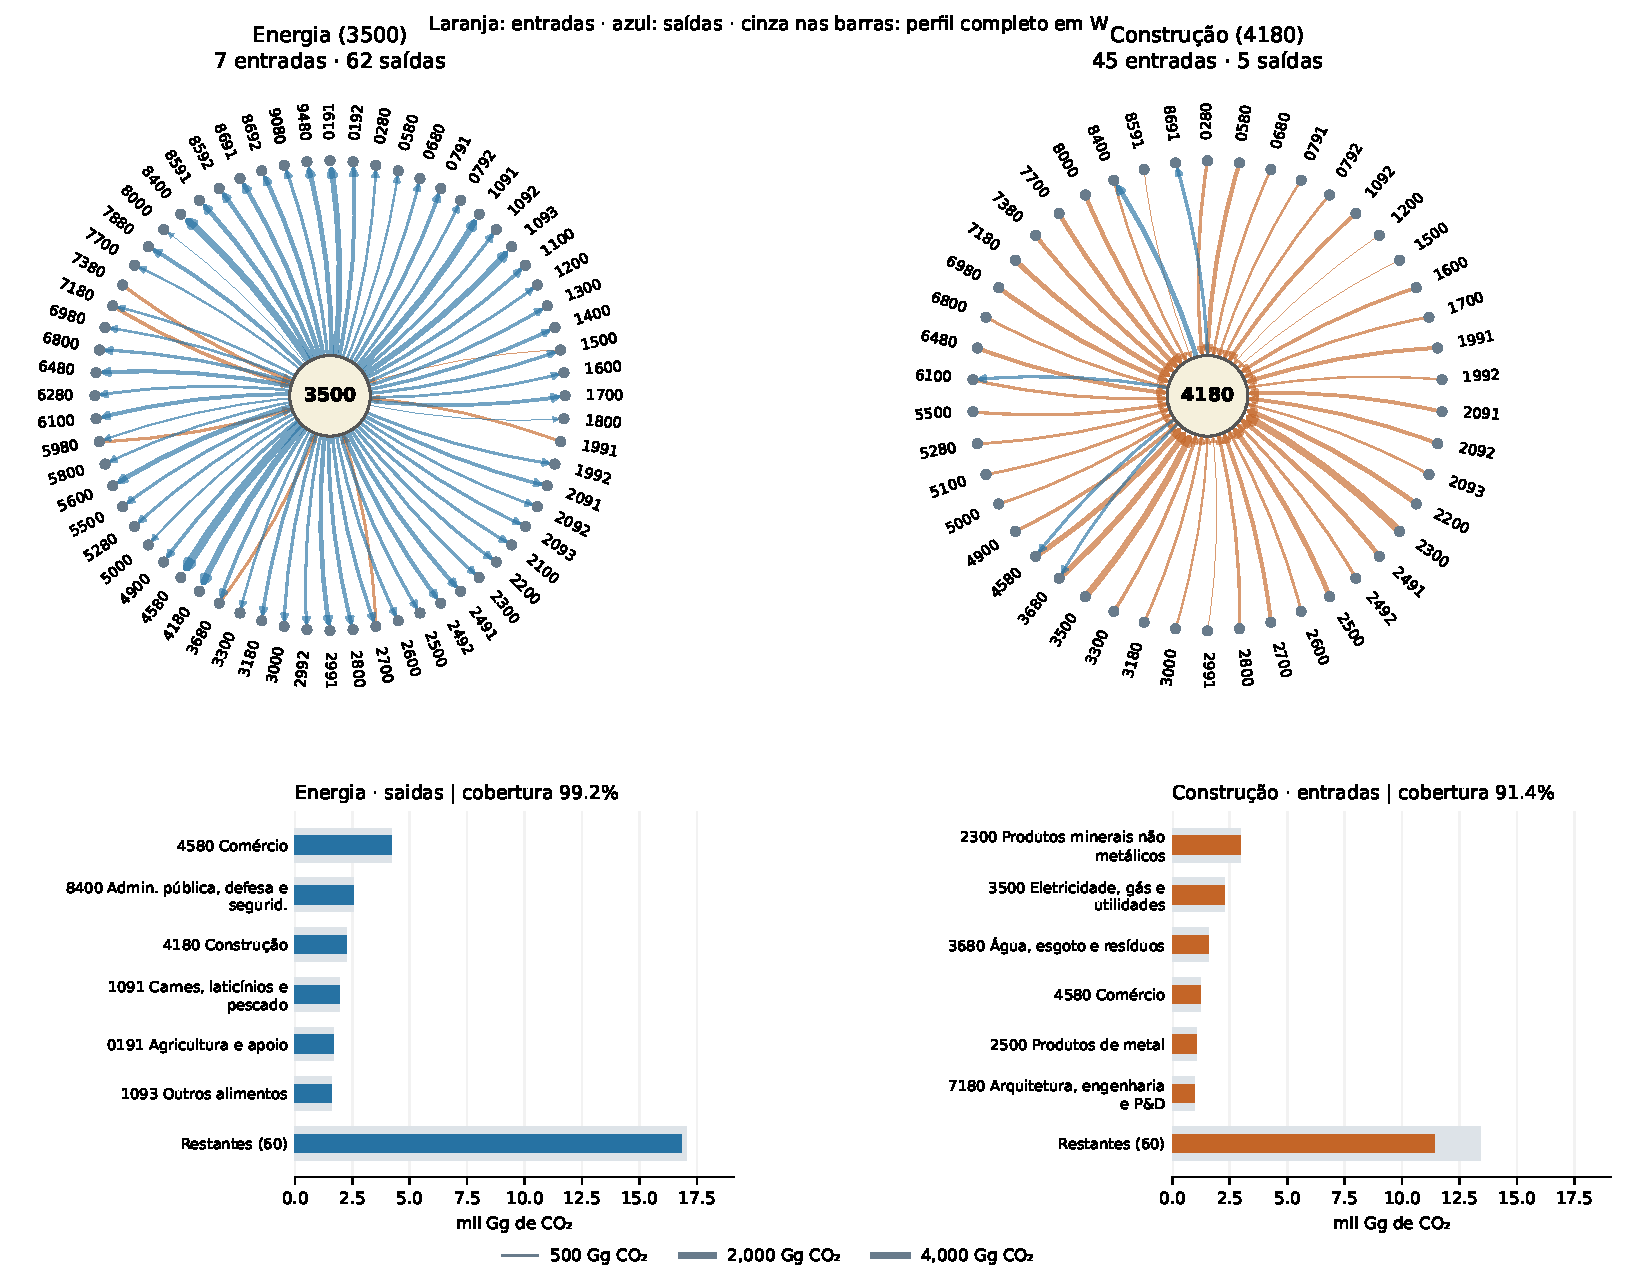
\includegraphics[width=0.96\linewidth,height=0.70\textheight,keepaspectratio]{figuras/artigo_relacoes_combinada.pdf}
\end{center}
As redes são idênticas às da opção B. As barras repetem, sem recalcular, as saídas de energia e entradas de construção da opção A. Cinza: W completa; azul: saídas retidas; laranja: entradas retidas. Seis maiores relações mais parcela restante; eixo em mil Gg de CO\textsubscript{2}.

Base comum: MIP brasileira de 2015, 67 atividades e intensidades aproximadas de Sanguinet e Azzoni (2024). Backbone em $\alpha=0{,}05$, pesos originais, sem diagonal. Coberturas entrada/saída: energia 42,1\%/99,2\%; construção 91,4\%/57,0\%.
\clearpage
\end{document}
